
\documentclass[10pt,aps,prc,twocolumn]{revtex4-1}

\usepackage{tabularx} 
\usepackage{graphicx} 
\usepackage{hyperref}  
\usepackage{amssymb}  
\usepackage{amsmath}  
\usepackage[]{units}

\bibliographystyle{apsrev4-1}

\begin{document}
\title{Avoiding Bias Bias In Model Selection For Proton Radius Extractions}
% a.k.a. How I Learned to Stop Worrying and Love the Bias

\author{Randall Evan McClellan}
\affiliation{Jefferson Lab, Newport News, VA 23606}
\author{Douglas Weadon Higinbotham}
\affiliation{Jefferson Lab, Newport News, VA 23606}
\author{Xuefei Yan}
\affiliation{Duke University, Durham, NC 27708}
\author{Simon \v{S}irca}
\affiliation{Jo\v{z}ef Stefan Institute, SI-1000 Jjubjana, Slovenia}
\author{Miha Mihovilovi\v{c}}
\affiliation{Jo\v{z}ef Stefan Institute, SI-1000 Jjubjana, Slovenia}

\begin{abstract}
Intuitively, a scientist might assume that a more complex statistical model will necessarily yield a more 
accurate description of experimental data.   Herein, we analyze this anzats in the context of extracting 
the proton charge radius from simulated charge form factor data.  We will show that, for a given set of data, 
a biased parsimonious model can in fact be the better predictive model.  Perhaps more surprising,
we will also show that in certain cases a simple parsimonious model can in fact be a better predictive model 
then even the generating function.   While illustrated for the case of radius extraction of electron scattering data,
this result provides an important example of the fact a scientist cannot achieve a better result by
over-parameterization.
\end{abstract}

\maketitle

\section{Introduction}

High precision muonic Lamb shift experiments have determined the proton radius to 
be 0.84087(39)~fm~\cite{Pohl:2010zza,Antognini:1900ns}.   This result is in stark contrast to the current
CODATA recommended value of 0.875~fm~\cite{Mohr:2015ccw} which comes from an average of atomic 
Lamb shift and electron scattering results.  

While initial efforts to understand this puzzle focused on the details of the muonic experiment, attention has
now turned to re-examining the atomic and electron scattering results.   In fact, the first of the
new generation of published atomic Lamb shift measurements is in statistical agreement with the muonic 
result~\cite{Beyer79} though preliminary results from another group agrees with the classic atomic 
results~\cite{fleurbaey:tel-01633631}.

For the electron scattering data, the proton's charge radius, $r_p$, is extracted from
cross section data by determining the slope of the electric form factor, $G_E$, in the
limit of four-moment transfer, $Q^2$, approaching zero: 
$$
  r_p \equiv \sqrt{ \langle r^2 \rangle}
   = \left( -6  \left. \frac{\mathrm{d} G_E(Q^2)}{\mathrm{d}Q^2}
    \right|_{Q^{2}=0} \right)^{1/2} \>.
$$
Of course, electron scattering cannot reach the exact $Q^2 = 0$ limit; thus,
an extrapolation is required to extract the charge radius from the experimental data.

Many methods have been proposed to make this extrapolation,
ranging from parsimonious fits of low $Q^2$ data~\cite{Griffioen:2015hta,Horbatsch:2016ilr,Higinbotham:2015rja} 
to extremely complex models with tens of free parameters~\cite{Bernauer:2013tpr,Lee:2015jqa}.   
As nicely illustrated in the work of Krauth~{\it{et al.}}~\cite{Krauth:2017ijq}, the 
parsimonious fits tend to agree with the muonic results while the more complex fits 
are generally in agreement with the CODATA value.

A general criticisms of the parsimonious extractions of the proton radius is the presence of bias~\cite{Sick:2017aor},
with an implication that bias needs to be avoided in order to successfully extract the true radius from the data.
In fact, the use of bias to reject statistical models dates back to the classic Monte Carlo study of Borkowski~{\it{et al.}}~\cite{Borkowski:1975}. 
We will show in this work that when using a Monte Carlo study to test a statistical model's ability
to extract the proton radius, one needs to only only consider bias but also the variance and
illustrate how a biased parsimonious model can in fact have a higher predictive validity than an 
unbiased less parsimonious model.

\section{Bias}

In the English language bias often used as pejorative term, while in the context of regression, it is simply
an offset from the ideal of a distribution.   It is important to note, that since it is part of a distribution it
is not a property of a single realization but determined by repeated sampling.    In the context of the proton 
radius extractions, bias was nicely illustrated by Borkowski~{\it{et al.}}~\cite{Borkowski:1975} and we will
following their procedure.

Randomly generate sets of pseudo charge form factor data in steps of $\unit[0.05]{fm^{-2}}$ from $\unit[0.1]{fm^{-2}}$ to 0.4, 0.8, 1.2,
and $\unit[1.6]{fm^{-2}}$ using the standard dipole function:
\begin{equation}
\label{sd}
G\mathrm{_D}(Q^2) = ( 1 + Q^2/(\unit[18.27]{fm^{-2}}))^{-2}.
\end{equation}
Perform fits on the resulting sets of pseudo data with linear and quadratic functions:
\begin{equation}
f_{linear}(Q^2) = a_0 + a_1 * Q^2
\end{equation}
\begin{equation}
f_{quadratic}(Q^2) = a_0 + a_1 Q^2 + a_2 Q^4 
\end{equation}
These functions are written so that they are linear in terms.  This allows the minimization to be solved exactly
and also allows the normalization to float is a common practice.   By factoring out the normalization term, a$_0$, 
the slope given by a$_1$/a$_0$ can be used to determine the radius.

This procedure was done with $10^6$ sets of randomized pseudo data to precisely determine the mean of the extracted 
radii for these two models.   Since we used standard dipole as the input function, one would expect an unbiased 
function to return a radius of 0.81fm.
Table~\ref{ztable} reproduces the table found in the
Z. Physik article and example code is provided in the supplemental material.
As the table clearly shows, the mean of linear fits shows a clear bias. 
Therefore, the authors conclude that the linear models should always be rejected in favor of the lower-bias quadratic function.
They then proceed to extract the proton charge radius from real data using a five parameter fit: a quadratic charge form factor 
and three floating normalizations.

\begin{table}
\caption{The following table shows the mean a$_0$ and radius terms from doing $10^6$ Monte Carlo simulations
for each range
where Eq.~\ref{sd} was used to generate faux data in $\unit[0.05]{fm^{-2}}$ steps with each points randomized using
0.5\% normal distribution.   The results clearly indicate that the linear fits are biased.   The input
radius was \unit[0.8113]{fm} (an a$_1$/a$_0$ term of $\unit[0.1097]{fm^{-1}}$) and an a$_0$ of one.}
\begin{tabular}{c|cc|cc} \hline
interval       & \multicolumn{2}{c|}{linear fit} & \multicolumn{2}{c}{quadratic fit}  \\
fm$^{-2}$      & a$_0$      & radius          & a$_0$    & radius \\ \hline
 0.1 -- 0.4 & 1.000& 0.79& 1.000& 0.81 \\
 0.1 -- 0.8 & 0.999& 0.78& 1.000& 0.81 \\
 0.1 -- 1.2 & 0.997& 0.77& 1.000& 0.81 \\
 0.1 -- 1.6 & 0.996& 0.76& 1.000& 0.81 \\ \hline
\end{tabular}
\label{ztable}
\end{table}

\section{Variance}

While the mean of the results is indeed correct; when we run an experiment we typically do no get to run it $10^6$ times.
In particular in nuclear physics, the experiments are few and far between thus we need to carefully consider variance as
well as the bias when picking the statistical model to use.

Table~\ref{fulltable} shows more complete picture of the simulation results where the variance is shown along with the bias.
This table in fact shows nearly a textbook illustration of the trade-off between variance and bias with the simple fits
having a relatively high bias with a low variance while the quadratic fits have a low bias and high variance.

\begin{table*}
\caption{The input radius was 0.8113 fm (an a1/a0 of $\unit[0.1097]{fm^{-1}}$).}
\begin{tabular}{cc|cccccc|cccccc} \hline
Data   & Range     & \multicolumn{6}{c|}{linear fit}                       & \multicolumn{6}{c}{quadratic fit}                    \\ 
Points & fm$^{-2}$ &   a$_0$  & Radius&  a$_1$/a$_0$ &  Bias  & Sigma &  RMSE  &   a$_0$  & Radius& a$_1$/a$_0$  &  Bias  & Sigma &  RMSE \\  \hline
7      & 0.1 -- 0.4 & 0.9995& 0.7948& -0.1053& -0.0044& 0.0184& 0.0189 & 1.0000& 0.8063& -0.1084& -0.0013& 0.1094& 0.1094\\
15     & 0.1 -- 0.8 & 0.9987& 0.7828& -0.1021& -0.0076& 0.0057& 0.0095 & 1.0000& 0.8096& -0.1092& -0.0005& 0.0281& 0.0281\\
22     & 0.1 -- 1.2 & 0.9975& 0.7712& -0.0991& -0.0106& 0.0030& 0.0110 & 0.9999& 0.8089& -0.1090& -0.0007& 0.0138& 0.0138\\
31     & 0.1 -- 1.6 & 0.9959& 0.7600& -0.0963& -0.0134& 0.0019& 0.0136 & 0.9998& 0.8075& -0.1087& -0.0010& 0.0085& 0.0085\\ \hline
\end{tabular}
\label{fulltable}
\end{table*}

\begin{figure}[htbp]
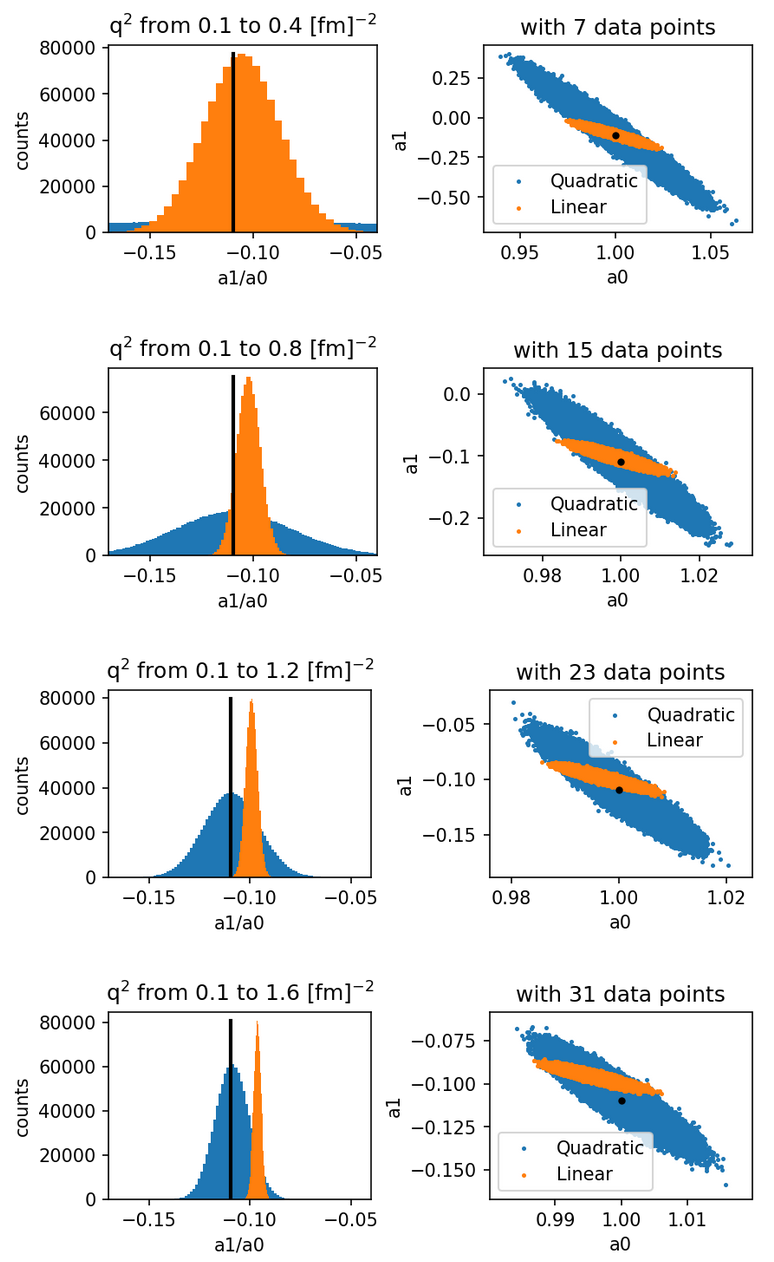
\includegraphics[width=\columnwidth]{Figure/zresult.png}
\caption{A graphic representation of the Monte Carlo results showing how the linear fits tend to have a relatively
high bias though a low variance while the quadratic fits tend to have a relatively low bias but a large variance.}
\end{figure}

\begin{table*}
\caption{Same as before, but now with equal number of data points of each range.}
\begin{tabular}{cc|cccccc|cccccc} \hline
Data   & Range     & \multicolumn{6}{c|}{linear fit}                       & \multicolumn{6}{c}{quadratic fit}                    \\ 
Points & fm$^{-2}$ &   a$_0$  & Radius&  a$_1$/a$_0$ &  Bias  & Sigma &  RMSE  &   a$_0$  & Radius& a$_1$/a$_0$  &  Bias  & Sigma &  RMSE \\  \hline
31& 0.1 - 0.4 & 0.9995& 0.7951& -0.1054& -0.0043& 0.0098& 0.0107 & 1.0000& 0.8090& -0.1091& -0.0006& 0.0629& 0.0629 \\
31& 0.1 - 0.8 & 0.9987& 0.7829& -0.1021& -0.0076& 0.0041& 0.0086 & 1.0000& 0.8099& -0.1093& -0.0004& 0.0208& 0.0208  \\
31& 0.1 - 1.2 & 0.9974& 0.7712& -0.0991& -0.0106& 0.0026& 0.0109 & 0.9999& 0.8089& -0.1091& -0.0006& 0.0121& 0.0121  \\
31& 0.1 - 1.6 & 0.9959& 0.7600& -0.0963& -0.0134& 0.0019& 0.0136 & 0.9998& 0.8076& -0.1087& -0.0010& 0.0085& 0.0085  \\  \hline
\end{tabular}
\label{equaldatatable}
\end{table*}

\section{Goldilocks Dilemma}

For any given set of statistical models, the goal is to find the optimal balance between bias and variance.   
As was noted by George Box, all models are wrong, thus the goal is to find the most appropriate one. 
In general, this can be written as,
\begin{equation}
\frac{d Bias^2 }{ d Complexity} = \frac{- d Variance }{ d Complexity }
\end{equation}

Thus going back to Table~\ref{fulltable} and checking the root mean square error, one can see that for the four ranges
one finds the 0.1 -- 0.8 range is actually optimal for the linear model and the 0.1 -- 1.6 range is optimal for the quadratic model. 
This is in complete contrast to the conclusion one draws when only considers bias as presented in Table~\ref{ztable}
though constant with the observation that the optimal specific form of the parameterization may depend on the $Q^2$ region
being fit~\cite{Alberico:2008sz}.
\begin{figure}
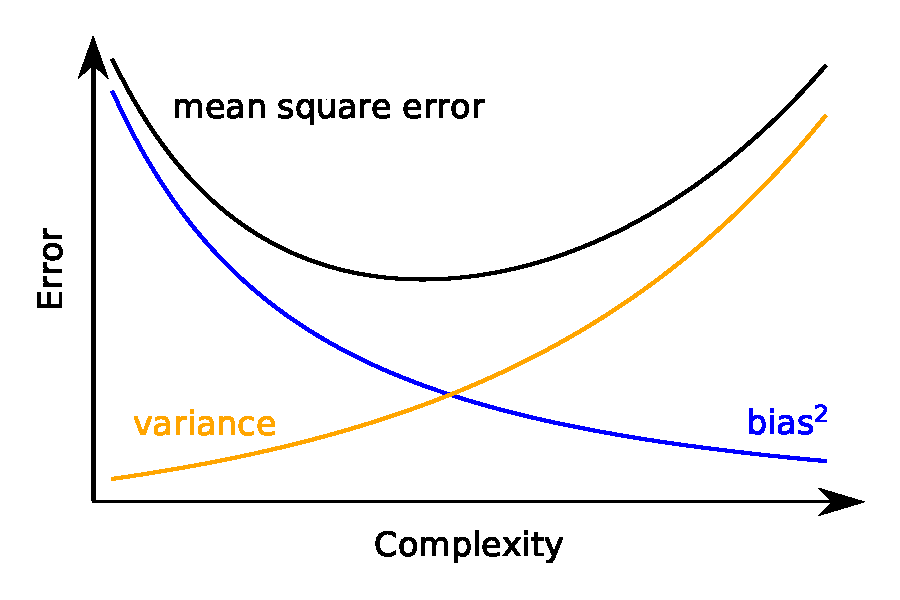
\includegraphics[width=\columnwidth]{Figure/biasvariance-clean.pdf}
\caption{An illustration of the trade-off between bias and variance when selecting a statistical model.   Simple models
will have low variance but high bias (under-fitting) while complex models will have low bias but high variance (over-fitting).   
It is this trade-off that one seeks to balance.   While with repeated  Monte Carlo simulations it is trivial to find the optimal
predictive model for a give set of data; in the real world true model is typically unknown and one only gets preform a very limited number
of experiments and thus one relies on using real data and statistical methods for model selection~\cite{Hastie:2009}.
}
\end{figure}

It is interesting to repeat the Monte Carlo simulation for equal number of data points within each range
especially since for elastic scattering cross sections are significantly higher as lower values of $Q^2$
and thus it is easy to get more low $Q^2$ data.

As shown in Table~\ref{equaldatatable}, the picture is even grayer as the root mean square error of the linear 
fit is nearly equal to the quadratic thus, assuming standard dipole was the true generating function,  experiments
with 31 data point and an uncertainty of 0.005 per point over a range of 0.1 to 0.8 and a different experiment
over a range of 0.1 to 1.6 would produce nearly identical if all other things were equal.

In this case, the choice of the parsimonious modeler to use the low $Q^2$ data would like be driven by the recognition that as $Q^2$ increases
the extraction of a charge form factor is complicated by the growing influence of the magnetic form factor while the use of the larger $Q^2$
range would likely be driven by a desire to form a more complete picture of the proton's structure 
(e.g. one may be interested in not only in the proton's radius but also higher order moments).

\begin{figure}
\label{zoptimized}
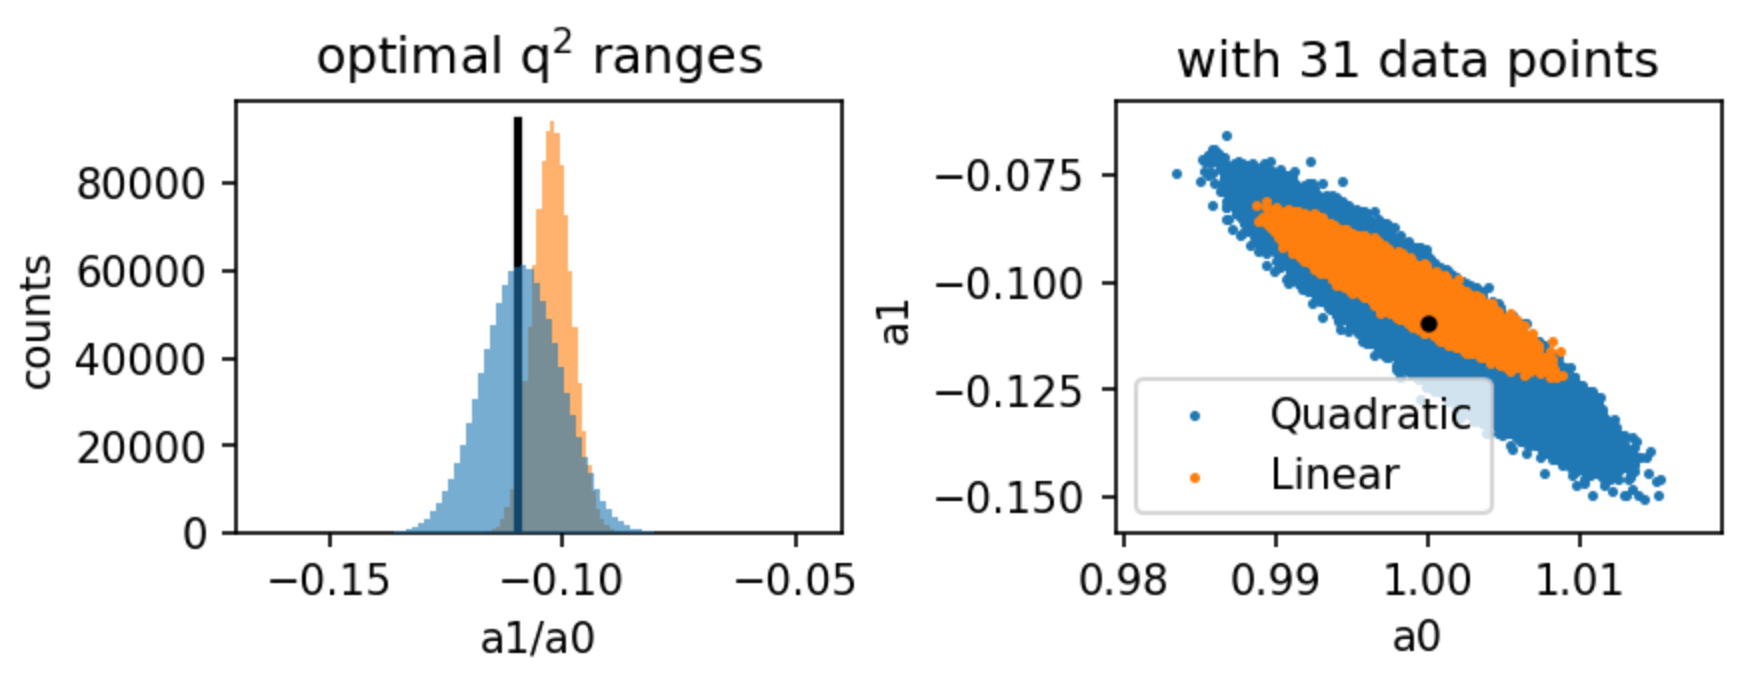
\includegraphics[width=\columnwidth]{Figure/zoptimized.png}
\caption{Shown is the result of million simulations and fits of linear fits  0.1 -- 0.8~fm$^{-2}$ 
and quadratic fits 0.1 -- 1.6~fm$^{-2}$ both with 31 equally spaced data points.    Using root mean
square error as the matrix, neither example is significantly better then the other for exacting the proton
radius   This is analogous to a dart game between two equally skilled players though one who hits the bulls eye more 
often yet has a large spread (low bias but high variance) and another equally skilled player who has a tighter cluster of hits
but an offset (high bias but low variance).}
\end{figure}


\section{The Best Predictive Model}

Selecting between a linear or quadratic regression of a more complex generating function may perhaps seems 
a bit contrived as one might naively think that just using the generating function itself would always yield the
best results.   To show that this is not in fact the case, 
we use the lowest Q$^2$ range, 0.1 - 0.4 fm$^{-2}$, and replace the quadratic function 
with the the generating function and a floating normalization term as follows:
\begin{equation}
f_{Dipole Fit}(Q^2) =  n_0 ( 1 - b_1 Q^2 / 2)^{-2}.
\end{equation}
where n$_0$ is the normalization term and an the radius will be given by $\sqrt{-6*b_1}$.
The results are shown in Table~\ref{simpleVSprefect} for a number of different random error as well as
for 0.05 and 0.005 fm$^{-2}$ spaces, the 7 and 61 points respectively.   While the linear fit always has
the greater bias, the dipole fit has the greater variance; bringing the root mean square error very close
together.   Notably, it takes 7 points with random errors less the 0.003 or 61 points with random error less
then 0.005 for the true function to be the better predictive regression model.

\begin{table*}
\caption{For the lowest range, 0.1 to 0.4 fm$^{-2}$ and continuing with a spacing of 0.05 (7 points) and 0.005 (61 points), 
it takes point-to-point random uncertainties at the 0.3\% level for fitting with the generating
functional form to provide a better predictive model then the simple linear fit.}
\begin{tabular}{cc|cccccc|cccccc} \hline
Data   & Random   & \multicolumn{6}{c|}{linear fit}                       & \multicolumn{6}{c}{dipole fit}            \\ 
Points & Error    & a$_0$ & Radius&a$_1$/a$_0$&  Bias  & Sigma &  RMSE  & n$_0$ & Radius& b$_1$  &  Bias  & Sigma &  RMSE   \\  \hline
%7      & 0.01     & 0.9995& 0.7941& -0.1051& -0.0046& 0.0359& 0.0361 & 1.0001& 0.8108& -0.1096& -0.0001& 0.0378& 0.0378  \\ 
7      & 0.005    & 0.9995& 0.7946& -0.1052& -0.0045& 0.0174& 0.0180 & 1.0000& 0.8114& -0.1097& -0.0000& 0.0194& 0.0194  \\
%7      & 0.003    & 0.9996& 0.7951& -0.1054& -0.0043& 0.0108& 0.0116 & 1.0000& 0.8114& -0.1097&  0.0000& 0.0114& 0.0114  \\
61     & 0.01     & 0.9995& 0.7949& -0.1053& -0.0044& 0.0135& 0.0142 & 1.0000& 0.8114& -0.1097&  0.0000& 0.0150& 0.0150  \\ 
%61     & 0.005     & 0.9995& 0.7952& -0.1054& -0.0043& 0.0069& 0.0081 & 1.0000& 0.8114& -0.1097&  0.0000& 0.0073& 0.0073  \\ \hline
\end{tabular}
\label{simpleVSperfect}
\end{table*}

The example with more points was added address if simply adding more points can justify using a more complex fit.
It is interesting to see that indeed by decreasing the spacing of the points
by one order of magnitude , leaving the point-to-point random error at 0.005, 
one can indeed get smaller RMSE from the input function, though size of the randon error is a critial parameter even
with 61 points as is seen in the 1\% case where linear becomes slightly better then true. 

Of course for real data, nature hides the true generating function from us, so perhaps is reassuring to know
that a reasonable approximation is able to reveal the underlying physics just as well if not better then the
true function..   A detailed description of the  behind the mathematics of this example problem can be 
found in {\it{To Explain or Predict}}~\cite{Shmueli:2010}.    

%
%To be clear, the lesson isn't that one funct one must find the most appropriate model for the task at hand.   
%

\section{Model Selection}

While this classic Monte Carlo example problem is over 40 years old, it actually points to exactly the split in 
the current electron scattering proton radius extraction procedures.     The parsimonious modelers, who are 
focused solely on extracting a radius, have focused in on the low $Q^2$ region accepting accepting a slightly higher 
level of bias in exchange for low variance while those modelers who are interesting in extracting more information 
about the proton (i.e. higher order moments) fit longer $Q^2$ ranges and have
focused on complex models which while lower in bias come at a cost of higher variance.  
It fact, the result of increasing $Q^2$ ranges requiring increasing complexity have resulted in
an uncertainty in the extracted radius 
stuck at $\approx \unit[0.01]{fm}$ since L.~Hand~\textit{et al.}'s original fit in 1963~\cite{Hand:1963zz}.

Also, since we don't know the true model, one cannot in general calculate the RMSE; so while Monte Carlo exercises 
like the one described herein are extremely useful for making sets are models; in the end, the data must be used 
to select the approximate model. 
For this one can relay on statistical modeling techniques such as chi2, reduced chi2, F-tests, A.I.C., B.I.C. 
to guide our selection of regression models and/or use theoretical constraints.

One should also always keep in mind that the input models in Monte Carlo simulations are always just an approximation
and one needs to be careful about drawing too strong an inference from the simulated results. 
For example, just because the linear model has a negative bias when compared to standard dipole, does not imply that 
it has a negative bias to all possible models.


\section{Summary}

For the specific example of electron scattering, we have revisited a classic Monte Carlo study and shown
the practice of simply concluding that an unbiased model will have the higher predictive validity 
is not a valid assumption; and in fact, one needs to consider both bias and variance when selecting
a predictive model.   This idea is in fact not constrained to the physical sciences, but also extends 
to quantitative analysis~\cite{Brighton:2015} and it at the heart of machine learning algorithms.
This important concept was nicely summarized by statistician George Box, ``Since all models 
are wrong the scientist cannot obtain a {\it{correct}} one
by excessive elaboration.  On the contrary, following William of Occam [s]he should seek an
economical description of natural phenomena. Just as the ability to devise simple 
but evocative models is the signature of the
great scientist so over-elaboration and over-parameterization is often
the mark of mediocrity.''~\cite{Box76}.


\section{Acknowledgments}

This work was supported by the U.S.  Department of Energy contract DE-AC05-06OR23177
under which Jefferson Science Associates operates the Thomas Jefferson National 
Accelerator Facility and contract DE-FG02-03ER4123 at Duke University.

\bibliography{elastic}

\end{document}
